\documentclass{article}
\usepackage[utf8]{inputenc}
\usepackage[T1]{fontenc}
\usepackage{geometry}
\usepackage{enumitem}
\usepackage{graphicx}

\geometry{margin=0.5in}

\begin{document}

\title{\textbf{Analog-to-Digital Converter \textit{(ADC)}}
\\ \large{Based on \textit{dr. inż. Maciej Dzieniakowski's knowledge}}}
\author{\textbf{Adrian Chmiel}}
\date{23 may 2024}
\maketitle

\section{Task}
The signal transmitted by the ADC converter controlled by switch A1 is fed \textit{(with a delay)} to the DAC converters and displayed on the oscilloscope screen.

\section{Configuration}
The configuration is divided into three main steps:
\begin{enumerate}[label=\arabic*.]
    \item \textbf{DAC converters configuration}
    \item \textbf{ADC converter configuration}
    \item \textbf{Setting switch A1 as an input channel}
\end{enumerate}
This division is also present in the rest of the document and it is recommended to follow this order to minimize encountered problems.

\section{Other remarks}
Firstly, we received a couple of advices that are worth mentioning at the beginning:
\begin{itemize}
    \item Proper ADC converter configuration is not an easy task, especially if we do that for the very first time
    \item The available ADC converter configuration allows for a lot of control over the signal through many available parameters
    \item The default values of the bits for each parameter are \textbf{0} which means that we do not always have to set them
\end{itemize}
It is recommended to follow the following scheme:
\vspace{3mm} \\
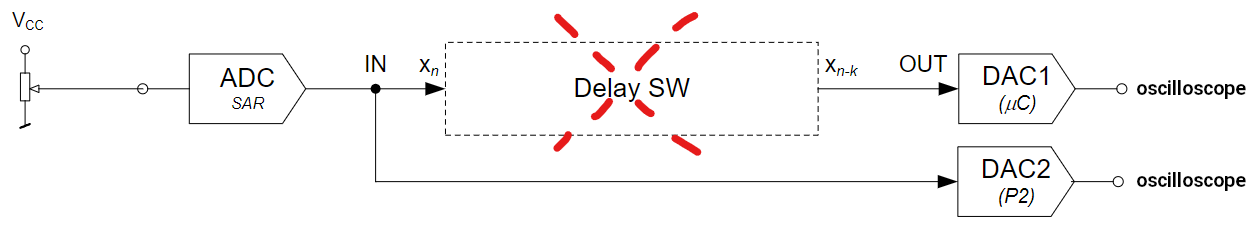
\includegraphics[width=\textwidth]{"../img/ADC_delay_DAC_eng.png"}
\textit{Source: ADC\_delay\_DAC.pdf, page: 1}
\vspace{3mm} \\
\textbf{\textit{Delay SW}} means software (in this case a code fragment) delaying the signal.
I marked this element with a dashed line to indicate that for now it is not important for us.
However, this does not mean that this software should not be included in the final version of the program.

\section{DAC converters configuration}
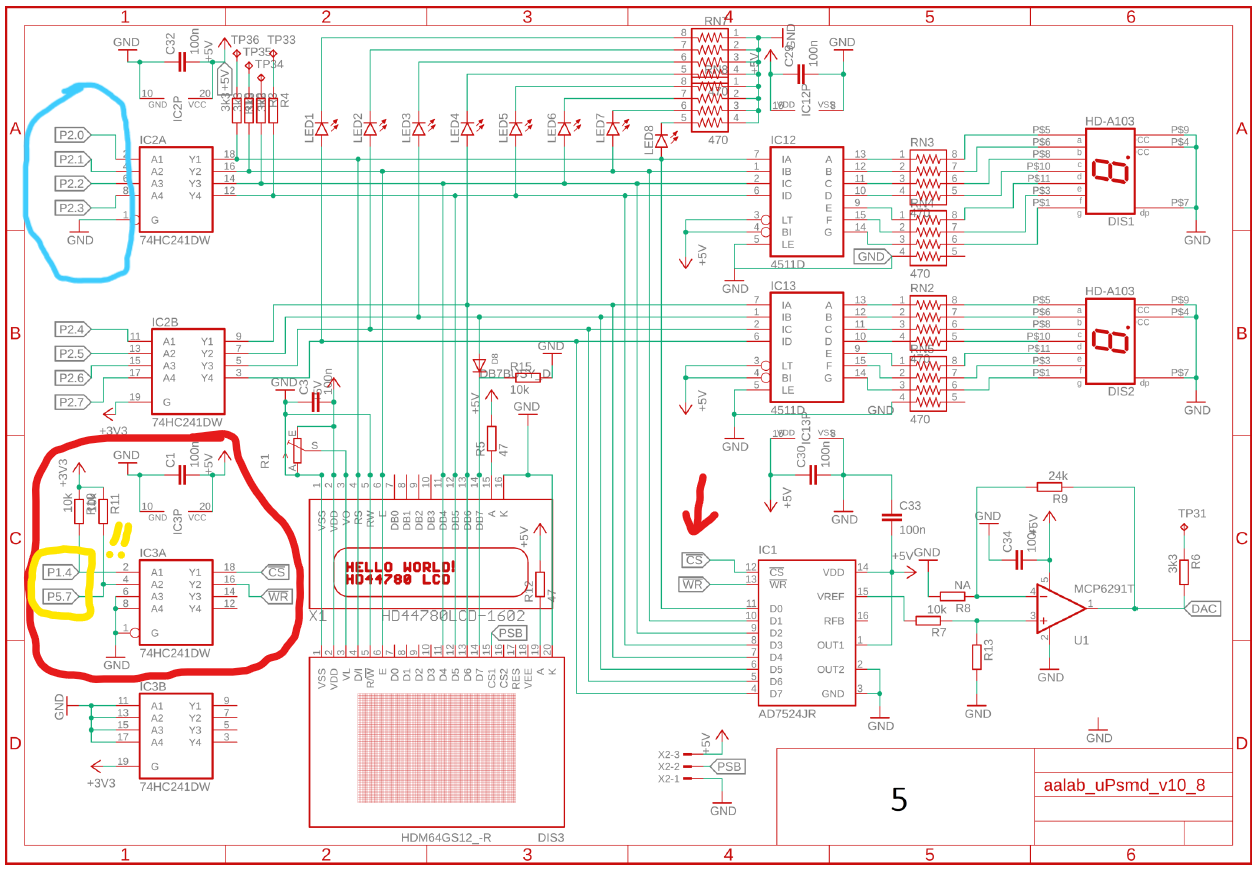
\includegraphics[width=\textwidth]{"../img/Blocks_scheme_7.png"}
\textit{Source: Blocks\_scheme.pdf, page: 7}
\vspace{3mm} \\
According to the above scheme, it is necessary to configure the \textit{P1.4} and \textit{P5.7} ports as \textbf{outputs} so that it is possible to view the results on the oscilloscope screen after connecting it to the appropriate pins.
In addition, it is necessary to set all pins from port \textit{P2} as \textbf{outputs}.
This can be done with the following code fragment in the initialization section:
\begin{verbatim}
    BIS.B #00010000b, &P1DIR ; set P1.4 as out
    BIS.B #10000000b, &P5DIR ; set P5.7 as out
    BIC.B #00010000b, &P1OUT ; clear bit P1.4
    BIC.B #10000000b, &P5OUT ; clear bit P5.7
    MOV.B #255, P2DIR        ; set all pins from port 2 as outputs
    MOV.B #0, P2OUT          ; set port 2 to low \end{verbatim}
The rest of the configuration can be done using the code we received during the \textbf{timer task}:
\newpage
\begin{verbatim}
     ;---------- Basic Clock Module Initialisation --------------------------------------
     ; - switch from DCO to XT2
     ; - MCLK & SMCLK supplied from XT2, ACLK = n/a
     ; - the DCO is left runing
     bis.b #OSCOFF,SR ;turn OFF osc.1
     bic.b #XT2OFF,BCSCTL1 ;turn ON osc.2
BCM0 bic.b #OFIFG,&IFG1 ;clear OFIFG
     mov #0FFFFh,R15 ;delay (waiting for oscilator start)
BCM1 dec R15 ;delay
     ;jnz BCM1 ;delay -> commented out as it was ocasionally leading to infinite loop
     bit.b #OFIFG,&IFG1 ;test OFIFG
     jnz BCM0 ;repeat test if needed
     ;MCLK
     bic.b #040h,&BCSCTL2 ;slelect XT2CLK as source
     bis.b #080h,&BCSCTL2 ;
     bic.b #030h,&BCSCTL2 ;MCLK=source/1 (8MHz)
     ;SMCLK
     bis.b #SELS,&BCSCTL2 ;slelect XT2CLK as source
     bic.b #006h,&BCSCTL2 ;SMCLK=source/1 (8MHz)
     ;---

     ;... ;DAC_0 initialisation 
     bis.w #REFON+REF2_5V,&ADC12CTL0 ;Reference generator ON, VRef+=2.5V
     bic #DAC12SREF0,&DAC12_0CTL ;set Vref=VREF+
     bic #DAC12SREF1,&DAC12_0CTL ;
     bic #DAC12RES,&DAC12_0CTL ;12-bit resolution
     bic #DAC12LSEL0,&DAC12_0CTL ;Load mode 0
     bic #DAC12LSEL1,&DAC12_0CTL ;
     bis #DAC12IR,&DAC12_0CTL ;Full-Scale=1xVref
     bis #DAC12AMP0,&DAC12_0CTL ;High speed amplifier output 
     bis #DAC12AMP1,&DAC12_0CTL ; 
     bis #DAC12AMP2,&DAC12_0CTL ;
     bic #DAC12DF,&DAC12_0CTL ;Data format - straight binary 
     bic #DAC12IE,&DAC12_0CTL ;Interrupt disabled 
     bis #DAC12ENC,&DAC12_0CTL ;DAC_0 conversion enabled 
     ;...

     ;... ;DAC_1 initialisation 
     bis.w #REFON+REF2_5V,&ADC12CTL0 ;Reference generator ON, VRef+=2.5V
     bic #DAC12SREF0,&DAC12_1CTL ;set Vref=VREF+
     bic #DAC12SREF1,&DAC12_1CTL ;
     bic #DAC12RES,&DAC12_1CTL ;12-bit resolution
     bic #DAC12LSEL0,&DAC12_1CTL ;Load mode 0
     bic #DAC12LSEL1,&DAC12_1CTL ;
     bis #DAC12IR,&DAC12_1CTL ;Full-Scale=1xVref
     bis #DAC12AMP0,&DAC12_1CTL ;High speed amplifier output 
     bis #DAC12AMP1,&DAC12_1CTL ; 
     bis #DAC12AMP2,&DAC12_1CTL ;
     bic #DAC12DF,&DAC12_1CTL ;Data format - straight binary 
     bic #DAC12IE,&DAC12_1CTL ;Interrupt disabled 
     bis #DAC12ENC,&DAC12_1CTL ;DAC_1 conversion enabled 
     ;... \end{verbatim}

\section{ADC converters configuration}
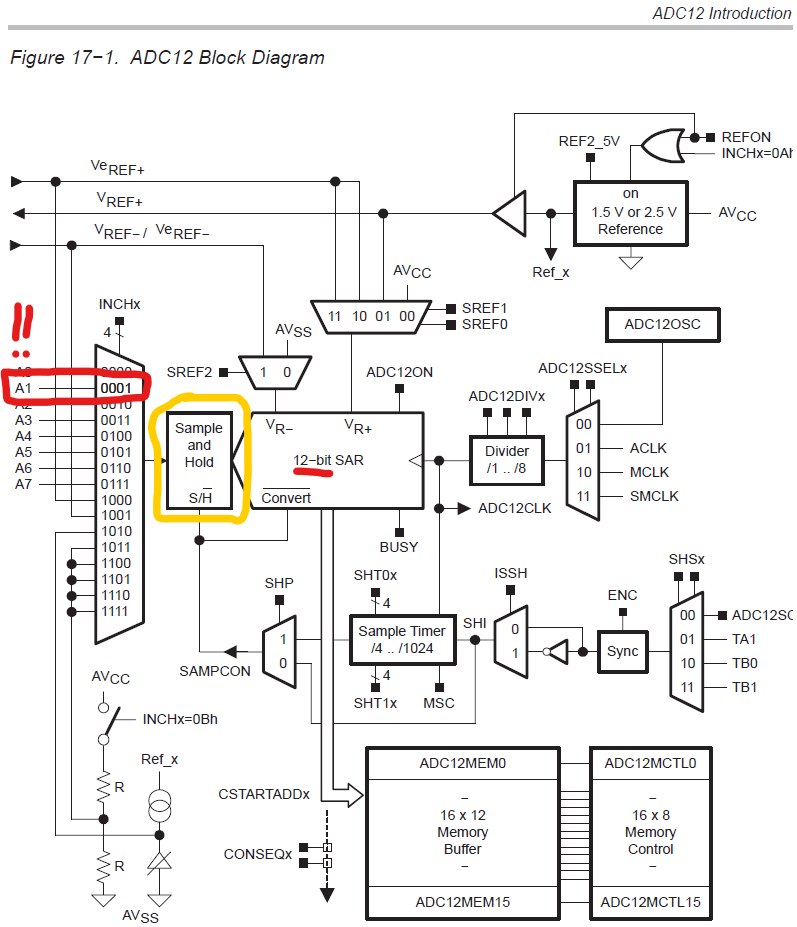
\includegraphics[width=\textwidth]{"../img/slau049f_346.png"} \\
\textit{Source: slau049f.pdf, page: 346}
\newpage
The ADC converter configuration is a bit more complicated than the DAC converters configuration. It is worth paying attention to a couple of aspects:
\begin{itemize}
    \item The ADC converter is \textbf{12-bit}, but in reality we are only interested in the \textbf{8 least significant bits}, because one of the used DAC converters is only \textbf{8-bit}.
    \item The \textit{Sample and Hold} parameter allows you to take a sample and hold it - this is necessary for the converter to work correctly with a delay.
\end{itemize}
The entire configuration process can be divided into three steps:
\begin{enumerate}[label=\arabic*.]
    \item \textbf{Initial configuration of ADC12CTL0}
\vspace{3mm} \\
The documentation corresponding to this step is below: \\
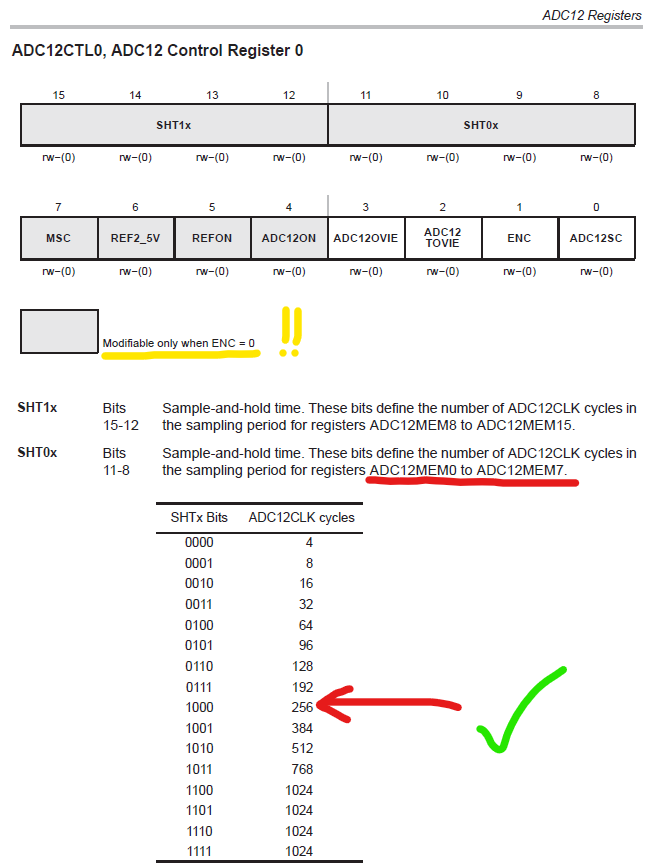
\includegraphics[width=0.775\textwidth]{"../img/slau049f_364.png"} \\
\textit{Source: slau049f.pdf, page: 364}
\vspace{3mm} \\
Due to the fact that we will only deal with 8-bit numbers, we only need cells \textit{ADC12MEM0 - ADC12MEM7}.
Therefore, it is enough to set only the sample holding time \textit{SHT0} corresponding to these cells. The recommended time is \textbf{256 clock cycles}! \\
\vspace{3mm} \\
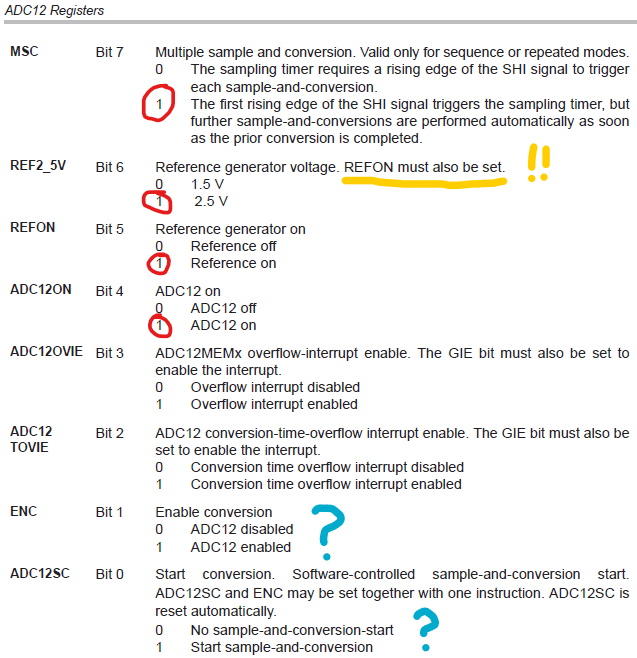
\includegraphics[width=0.875\textwidth]{"../img/slau049f_365.png"} \\
\textit{Source: slau049f.pdf, page: 365}
\vspace{3mm} \\
This part requires a thorough understanding of the above documentation fragment, as we change quite a few parameters here.
\begin{itemize}
     \item \textit{MSC} - allows the next conversions to be performed automatically one after the other
     \item \textit{REF2\_5V} - we set the reference voltage to 2.5V
     \item \textit{REFON} - we turn on the reference voltage generator
     \item \textit{ADC12ON} - we turn on the ADC converter
     \item \textit{ADC12OVIE \& ADC12TOVIE} - correspond to the interrupt, which we will not use, so the bit value remains unchanged
     \item \textit{ENC} - allows conversion \textbf{(set only at the end of the entire configuration!)}
     \item \textit{ADC12SC} - start conversion \textbf{(set only at the end of the entire configuration!)}
\end{itemize}
The code performing this step is available below:
\begin{verbatim}
BIS.W #0000100011110000b, &ADC12CTL0
; SHT0 = 1000b (256 cycles) | MSC = 1 | REF2_5V = 1 | REFON = 1 | ADC12ON = 1 \end{verbatim}
    \item \textbf{ADC12CTL1 configuration}
    \vspace{3mm} \\
The documentation corresponding to this step is below: \\
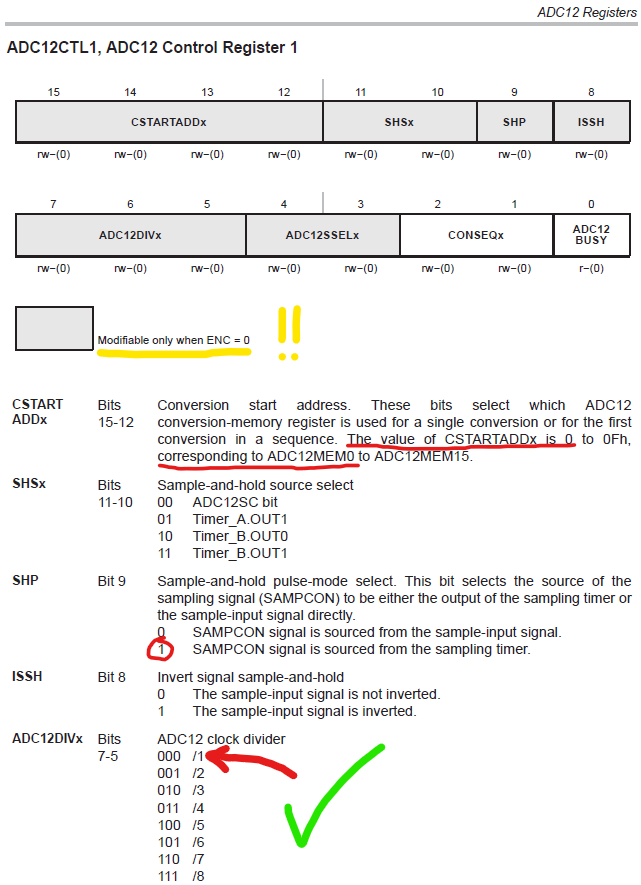
\includegraphics[width=0.825\textwidth]{"../img/slau049f_366.png"} \\
\textit{Source: slau049f.pdf, page: 366}
\vspace{3mm} \\
The following parameters are important in this step:
\begin{itemize}
     \item \textit{CSTARTADDx} - this is the address where the conversion result will start being saved - we leave it unchanged, so it will be \textit{ADC12MEM0}
     \item \textit{SHP} - allows an external signal to control the conversion (i.e. in our case \textbf{switch A1})
     \item \textit{ADC12DIVx} - this value divides the clock that the converter works with - we leave it unchanged to not change the clock frequency, but it is worth noting that this is a parameter that can be changed depending on the needs
\end{itemize}
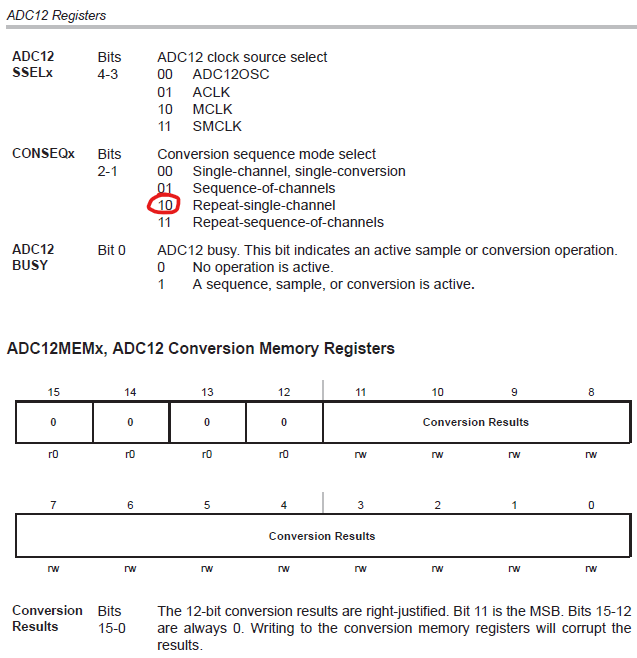
\includegraphics[width=0.9\textwidth]{"../img/slau049f_367.png"} \\
\textit{Source: slau049f.pdf, page: 367}
\vspace{3mm} \\
We change the \textit{CONSEQx} parameter to \textbf{10} so that the conversion is \textbf{repeated} based on a \textbf{single} channel with the A1 converter.
The code performing the entire step with the \textit{ADC12CTL1} configuration is below:
\begin{verbatim}
BIS.W #0000001000000010b, &ADC12CTL1
; SHP = 1 | CONSEQ2 = 1 -> A1 goes to MEM0 \end{verbatim}
\newpage
    \item \textbf{ADC12MCTL0 configuration}
     \vspace{3mm} \\
The documentation corresponding to this step is below: \\
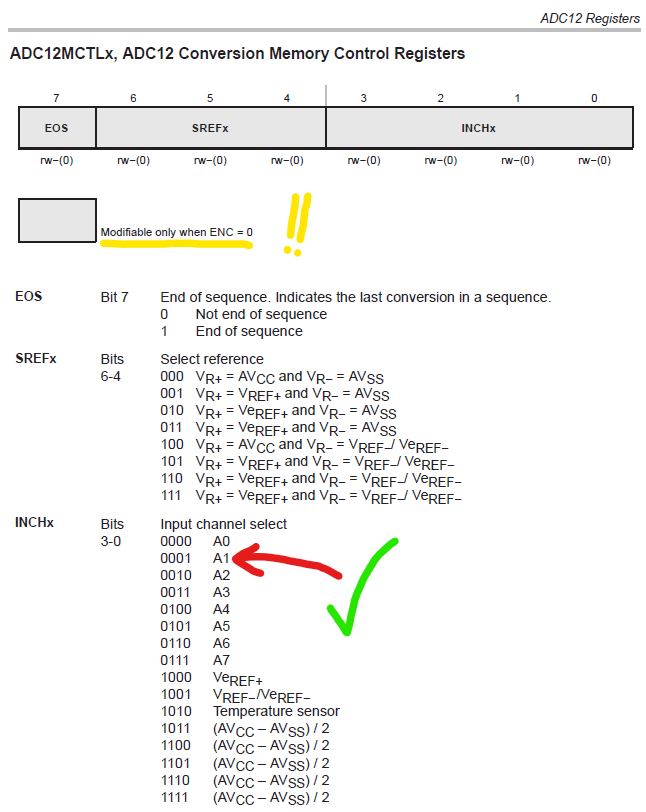
\includegraphics[width=0.9\textwidth]{"../img/slau049f_368.png"} \\
\textit{Source: slau049f.pdf, page: 368}
\vspace{3mm} \\
The only thing we do in this step is to set the input channel to \textbf{A1}, which will allow the switch to work correctly.
This is achieved by setting the \textit{INCHx} register to \textbf{0001}. The code performing this configuration is below:
\begin{verbatim}
BIS.B #00000001b, &ADC12MCTL0 ; set input channel as A1 \end{verbatim}
     \item \textbf{Allowing conversion and starting it}
     \vspace{3mm} \\
We return to the \textit{ADC12CTL0} configuration. This step must be done as the last element of the configuration, as it prevents the change of most of the other settings modified earlier.
To do this, we change the values of the \textit{ENC} and \textit{ADC12SC} registers to \textbf{1}.
\vspace{3mm} \\
The code performing this step is below:
\begin{verbatim}
BIS.W #11b, &ADC12CTL0 ; has to be at the end
; ENC = 1 | ADC12SC = 1 -> enables and starts conversion \end{verbatim}
\end{enumerate}

\section{Setting switch A1 as an input channel}
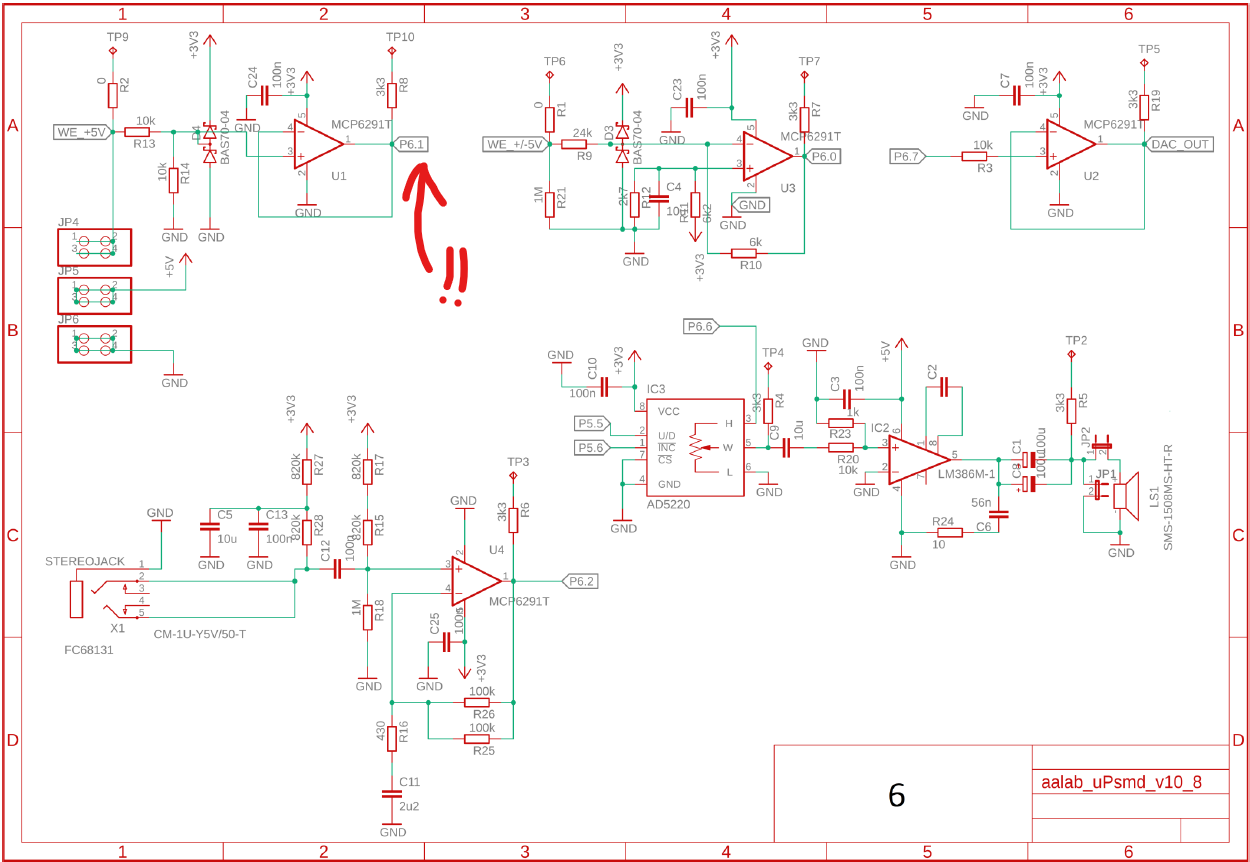
\includegraphics[width=\textwidth]{"../img/Blocks_scheme_8.png"}
\textit{Source: Blocks\_scheme.pdf, page: 8}
We have already partially done this task in the previous steps, but just like in the case of the converters above, it is necessary to set certain bits to specific values.
In this case, it is necessary to set the \textit{P6.1} port as an \textbf{analog input} with the \textit{P6SEL} register using the following code:
\begin{verbatim}
BIS.B #10b, &P6SEL ; set P6.1 as analog input \end{verbatim}
This fact can be supported by a fragment of the documentation below: \\
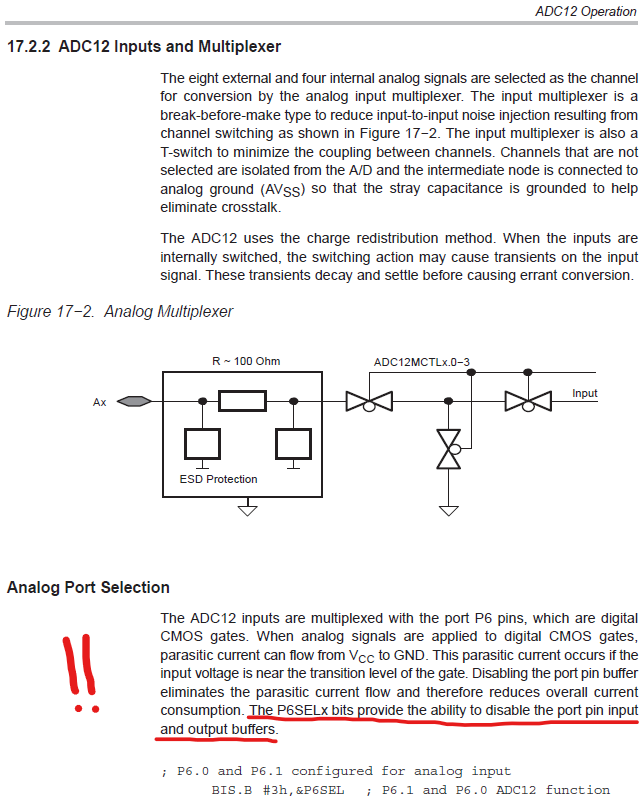
\includegraphics[width=0.9\textwidth]{"../img/slau049f_348.png"} \\
\textit{Source: slau049f.pdf, page: 348}

\newpage
\section{Final code with the entire configuration}
Complete code of the program with the configuration is visible below.
\begin{verbatim}
#include "msp430.h"                  ; #define controlled include file
 
     NAME    main                    ; module name

     PUBLIC  main                    ; make the main label vissible
                                     ; outside this module
     ORG     0FFECh
     DC16    TIMER_A0_Interrupt
     ORG     0FFFEh                  
     DC16    init                    ; set reset vector to 'init' label

     RSEG    CSTACK                  ; pre-declaration of segment
     RSEG    CODE                    ; place program in 'CODE' segment

init:   MOV     #SFE(CSTACK), SP        ; set up stack
     ; DAC_2 (P2) config
     BIS.B #00010000b, &P1DIR ; set P1.4 as out
     BIS.B #10000000b, &P5DIR ; set P5.7 as out
     BIC.B #00010000b, &P1OUT ; clear bit P1.4
     BIC.B #10000000b, &P5OUT ; clear bit P5.7
     MOV.B #255, P2DIR        ; set all pins from port 2 as outputs
     MOV.B #0, P2OUT          ; set port 2 to low

     ; ADC config (based on documentation)
     BIS.W #0000100011110000b, &ADC12CTL0
     ; SHT0 = 1000b (256 cycles) | MSC = 1 | REF2_5V = 1 | REFON = 1 | ADC12ON = 1
     BIS.W #0000001000000010b, &ADC12CTL1
     ; SHP = 1 | CONSEQ2 = 1 -> A1 forwarded to MEM0
     BIS.B #00000001b, &ADC12MCTL0 ; set input channel as A1
     BIS.B #10b, &P6SEL ; set P6.1 as analog input
     BIS.W #11b, &ADC12CTL0 ; has to be at the end
     ; ENC = 1 | ADC12SC = 1 -> enables and starts conversion

     ;---------- Basic Clock Module Initialisation --------------------------------------
     ; - switch from DCO to XT2
     ; - MCLK & SMCLK supplied from XT2, ACLK = n/a
     ; - the DCO is left runing
     bis.b #OSCOFF,SR ;turn OFF osc.1
     bic.b #XT2OFF,BCSCTL1 ;turn ON osc.2
BCM0 bic.b #OFIFG,&IFG1 ;clear OFIFG
     mov #0FFFFh,R15 ;delay (waiting for oscilator start)
BCM1 dec R15 ;delay
     ;jnz BCM1 ;delay -> commented out as it was ocasionally leading to infinite loop
     bit.b #OFIFG,&IFG1 ;test OFIFG
     jnz BCM0 ;repeat test if needed
     ;MCLK
     bic.b #040h,&BCSCTL2 ;slelect XT2CLK as source
     bis.b #080h,&BCSCTL2 ;
     bic.b #030h,&BCSCTL2 ;MCLK=source/1 (8MHz)
     ;SMCLK
     bis.b #SELS,&BCSCTL2 ;slelect XT2CLK as source
     bic.b #006h,&BCSCTL2 ;SMCLK=source/1 (8MHz)
     ;---

     ;... ;DAC_0 initialisation 
     bis.w #REFON+REF2_5V,&ADC12CTL0 ;Reference generator ON, VRef+=2.5V
     bic #DAC12SREF0,&DAC12_0CTL ;set Vref=VREF+
     bic #DAC12SREF1,&DAC12_0CTL ;
     bic #DAC12RES,&DAC12_0CTL ;12-bit resolution
     bic #DAC12LSEL0,&DAC12_0CTL ;Load mode 0
     bic #DAC12LSEL1,&DAC12_0CTL ;
     bis #DAC12IR,&DAC12_0CTL ;Full-Scale=1xVref
     bis #DAC12AMP0,&DAC12_0CTL ;High speed amplifier output 
     bis #DAC12AMP1,&DAC12_0CTL ; 
     bis #DAC12AMP2,&DAC12_0CTL ;
     bic #DAC12DF,&DAC12_0CTL ;Data format - straight binary 
     bic #DAC12IE,&DAC12_0CTL ;Interrupt disabled 
     bis #DAC12ENC,&DAC12_0CTL ;DAC_0 conversion enabled 
     ;...

     ;... ;DAC_1 initialisation 
     bis.w #REFON+REF2_5V,&ADC12CTL0 ;Reference generator ON, VRef+=2.5V
     bic #DAC12SREF0,&DAC12_1CTL ;set Vref=VREF+
     bic #DAC12SREF1,&DAC12_1CTL ;
     bic #DAC12RES,&DAC12_1CTL ;12-bit resolution
     bic #DAC12LSEL0,&DAC12_1CTL ;Load mode 0
     bic #DAC12LSEL1,&DAC12_1CTL ;
     bis #DAC12IR,&DAC12_1CTL ;Full-Scale=1xVref
     bis #DAC12AMP0,&DAC12_1CTL ;High speed amplifier output 
     bis #DAC12AMP1,&DAC12_1CTL ; 
     bis #DAC12AMP2,&DAC12_1CTL ;
     bic #DAC12DF,&DAC12_1CTL ;Data format - straight binary 
     bic #DAC12IE,&DAC12_1CTL ;Interrupt disabled 
     bis #DAC12ENC,&DAC12_1CTL ;DAC_1 conversion enabled 
     ;... 

main:   NOP                             ; main program
     MOV.W   #WDTPW+WDTHOLD,&WDTCTL  ; Stop watchdog timer
     mov.w   #0x5,&TACCR0            ; Period for up mode
     mov.w   #CCIE,&TACCTL0          ; Enable interrupts on Compare 0
     mov.w   #MC_1|ID_3|TASSEL_2|TACLR,&TACTL
     bis.w   #GIE,SR                 ; Enable interrupts (just TACCR0)

Mainloop:
     nop                             ; Required only for debugger
     JMP $                           ; jump to current location '$'                                       
                                     ; (endless loop)

TIMER_A0_Interrupt:
     MOV.W  &ADC12MEM0, R5           ; moving the value from ADC to R5
     MOV    R5, &DAC12_1DAT          ; moving that value to converter DAC_1 
     MOV.B  R5, &P2OUT               ; moving that value to converter DAC_2
     RETI

     END\end{verbatim}
\end{document}